% !TEX root = ../../prj4projektrapport.tex
% SKAL STÅ I TOPPEN AF ALLE FILER FOR AT MASTER-filen KOMPILERES 
\newpage
\section{Blok defintionsdiagram}

I dette afsnit ses blok definitionsdiagrammet for Spændingsregulator. Se figur \ref{fig:BDDSpaendingsregulator}. BDD'et er lavet for at give et overordnet indblik i de blokke, systemet består af.

\begin{figure}[H] % (alternativt [H])
	\centering
	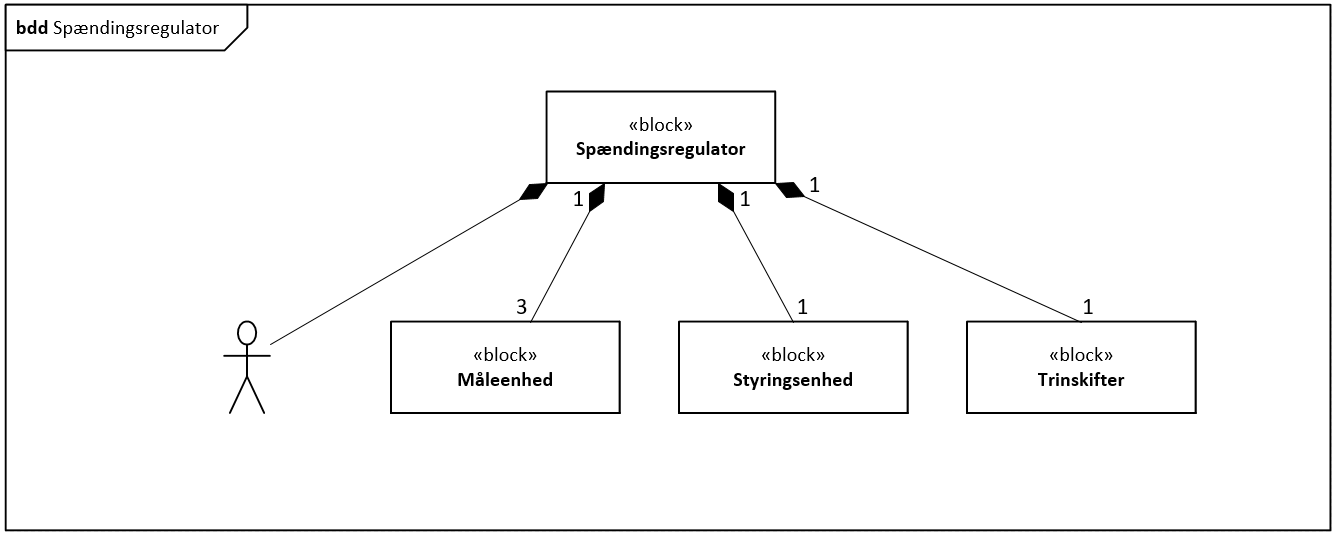
\includegraphics[width=0.9\textwidth]{Figure/BDDSpaendingsregulator}
	\caption{BDD Spændingsregulator}
	\label{fig:BDDSpaendingsregulator}
\end{figure}

Der arbejdes med tre overordnede blokke; Måleenhed, Styringsenhed og Trinskifter. Med udgangspunkt i MoSCoW er opgaverne, hver blok skal løse, beskrevet herunder:


Måleenheden skal kunne måle spænding, strøm, power factor og harmoniske, både centralt og decentralt. Data herfra skal kommunikeres videre til Styringsenheden. 


Styringsenheden skal kunne vise data på en skærm og burde kunne regulere Trinskifter automatisk. Der skal være muligheder for at regulere Trinskifter manuelt fra Styringsenheden. Den skal have et interface til kommunikation med Måleenheden. Det er derfor besluttet, at Styringsenhed har tre underblokke; Brugergrænseflade, Kontrolmodul og Kommunikationsmodul.


Trinskifter skal bestå af en trintransformer 24/0-8V og skal tilkobles en simuleret Distributionslinje og flere forbrugere. Derudover skal den indeholde en form for styring til trintransformeren.


For yderligere forklaring af blokkene se dokumentationen\footnote{Projektdokumentation, 5.1, Blok defintionsdiagram}.